\documentclass[border=10pt]{standalone}
\usepackage{pgfplots}
\pgfplotsset{compat=1.18}
\begin{document}
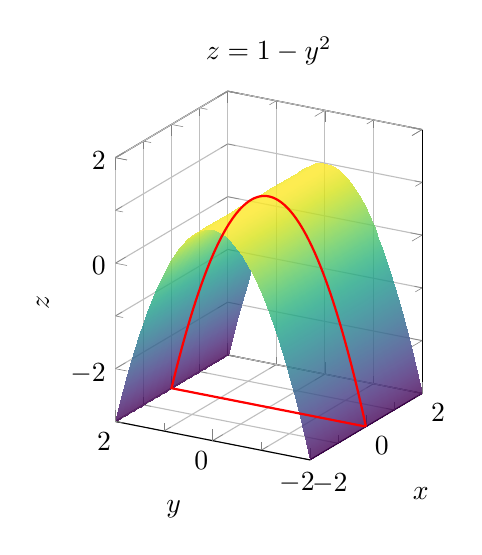
\begin{tikzpicture}
\begin{axis}[
    xlabel={$x$}, ylabel={$y$}, zlabel={$z$},
    title={$z = 1 - y^2$},
    view={-60}{20},
    colormap/viridis,
    samples=50, samples y=50,
    domain=-2:2, y domain=-2:2,
    zmin=-3, zmax=2,
    axis equal image,
    grid=both,
    minor tick num=1
]
\addplot3[surf, opacity=0.8, shader=interp] {1 - y^2};
\addplot3[red, thick, domain=-2:2, samples=100] (0, x, {1 - x^2});
\end{axis}
\end{tikzpicture}
\end{document}
